\documentclass[journal]{vgtc}                % final (journal style)
%\documentclass[review,journal]{vgtc}         % review (journal style)
%\documentclass[widereview]{vgtc}             % wide-spaced review
%\documentclass[preprint,journal]{vgtc}       % preprint (journal style)
%\documentclass[electronic,journal]{vgtc}     % electronic version, journal

%% Uncomment one of the lines above depending on where your paper is
%% in the conference process. ``review'' and ``widereview'' are for review
%% submission, ``preprint'' is for pre-publication, and the final version
%% doesn't use a specific qualifier. Further, ``electronic'' includes
%% hyperreferences for more convenient online viewing.

%% Please use one of the ``review'' options in combination with the
%% assigned online id (see below) ONLY if your paper uses a double blind
%% review process. Some conferences, like IEEE Vis and InfoVis, have NOT
%% in the past.

%% Please note that the use of figures other than the optional teaser is not permitted on the first page
%% of the journal version.  Figures should begin on the second page and be
%% in CMYK or Grey scale format, otherwise, colour shifting may occur
%% during the printing process.  Papers submitted with figures other than the optional teaser on the
%% first page will be refused.

%% These three lines bring in essential packages: ``mathptmx'' for Type 1
%% typefaces, ``graphicx'' for inclusion of EPS figures. and ``times''
%% for proper handling of the times font family.

\usepackage{mathptmx}
\usepackage{graphicx}
\usepackage{times}

\newcommand{\etal}{\emph{et~al.~}}

%% We encourage the use of mathptmx for consistent usage of times font
%% throughout the proceedings. However, if you encounter conflicts
%% with other math-related packages, you may want to disable it.

%% This turns references into clickable hyperlinks.
\usepackage[bookmarks,backref=true,linkcolor=black]{hyperref} %,colorlinks
\hypersetup{
  pdfauthor = {Josua Krause},
  pdftitle = {Visualizing Bike Share Traffic},
  pdfsubject = {},
  pdfkeywords = {},
  colorlinks=true,
  linkcolor= black,
  citecolor= black,
  pageanchor=true,
  urlcolor = black,
  plainpages = false,
  linktocpage
}

%% If you are submitting a paper to a conference for review with a double
%% blind reviewing process, please replace the value ``0'' below with your
%% OnlineID. Otherwise, you may safely leave it at ``0''.
\onlineid{0}

%% declare the category of your paper, only shown in review mode
\vgtccategory{Research}

%% allow for this line if you want the electronic option to work properly
\vgtcinsertpkg

%% In preprint mode you may define your own headline.
%\preprinttext{To appear in an IEEE VGTC sponsored conference.}

%% Paper title.

\title{Visualizing Bike Share Traffic}

%% This is how authors are specified in the journal style

%% indicate IEEE Member or Student Member in form indicated below
\author{Josua Krause}
\authorfooter{
%% insert punctuation at end of each item
}

%other entries to be set up for journal
\shortauthortitle{Krause: Visualizing Bike Share Traffic}
%\shortauthortitle{Firstauthor \MakeLowercase{\textit{et al.}}: Paper Title}

%% Abstract section.
\abstract{
% TODO
} % end of abstract

%% Keywords that describe your work. Will show as 'Index Terms' in journal
%% please capitalize first letter and insert punctuation after last keyword
\keywords{
Origin-destination data, bike share, flows
}

%% ACM Computing Classification System (CCS). 
%% See <http://www.acm.org/class/1998/> for details.
%% The ``\CCScat'' command takes four arguments.

\CCScatlist{ % not used in journal version
 %\CCScat{K.6.1}{Management of Computing and Information Systems}%
%{Project and People Management}{Life Cycle};
 %\CCScat{K.7.m}{The Computing Profession}{Miscellaneous}{Ethics}
}

%% Uncomment below to include a teaser figure.
  \teaser{
  % TODO
 \centering
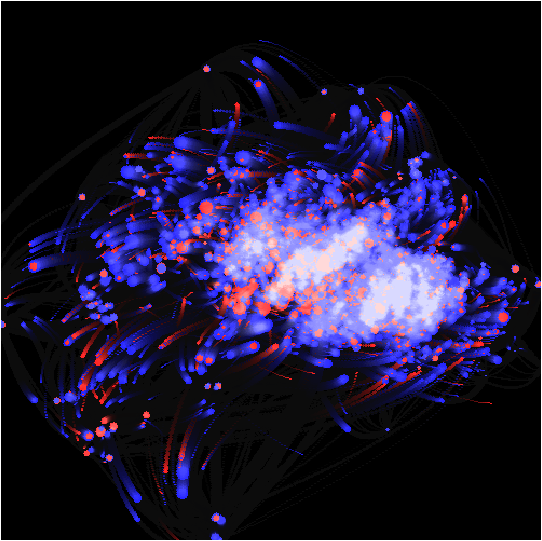
\includegraphics[width=3cm]{images/full_month_small.png}
\hspace*{0.5cm}
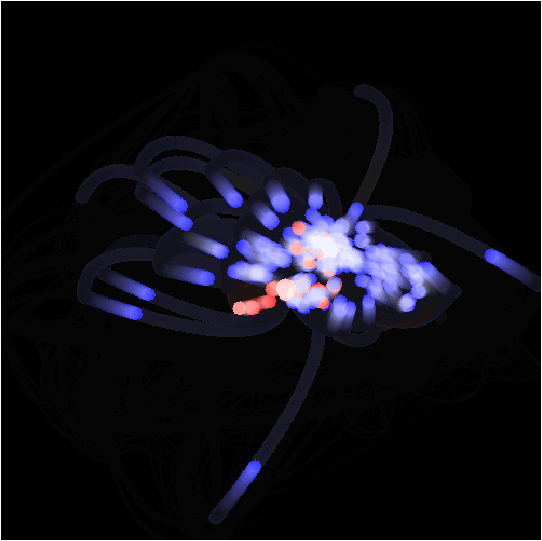
\includegraphics[width=3cm]{images/thresh_month_small.png}
\caption{One month worth of bike share users with and without thresholding aggregated journeys. Blue dots are subscribing bike share users and red dots are casual users.}
  }

%% Uncomment below to disable the manuscript note
%\renewcommand{\manuscriptnotetxt}{}

%% Copyright space is enabled by default as required by guidelines.
%% It is disabled by the 'review' option or via the following command:
% \nocopyrightspace

%%%%%%%%%%%%%%%%%%%%%%%%%%%%%%%%%%%%%%%%%%%%%%%%%%%%%%%%%%%%%%%%
%%%%%%%%%%%%%%%%%%%%%% START OF THE PAPER %%%%%%%%%%%%%%%%%%%%%%
%%%%%%%%%%%%%%%%%%%%%%%%%%%%%%%%%%%%%%%%%%%%%%%%%%%%%%%%%%%%%%%%%

\begin{document}

%% The ``\maketitle'' command must be the first command after the
%% ``\begin{document}'' command. It prepares and prints the title block.

%% the only exception to this rule is the \firstsection command
\firstsection{Introduction}

\maketitle

%% \section{Introduction} %for journal use above \firstsection{..} instead
Analyzing movement patterns of people is a task that just recently became
feasible. With the help of GPS trackers the daily routine of people can
be analyzed \cite{geo1, geo2, geo3}, although the number of participants
is limited. A larger number of trips can for example be acquired
by installing GPS trackers in taxi cabs \cite{Ferreira2013, Guo2012}.
With the inception of bike sharing programs in various cities large
amounts of journey data from people daily utilizing bicycles have
been automatically created.

For companies providing shared bicycles it is interesting to see who
uses the bikes, when they are used, and which routes have been taken.
For maintenance reasons it is also important to know whether the usage
of the bikes are balanced between stations or whether there are some
stations that are used more often as start or destination.
Tourists or one time users may produce such imbalances, so it
would be beneficial to detect whether casual users follow any patterns.
Since bike sharing is popular among commuters, using it daily to get
to work, it is interesting to see how the usage patterns change during
the rush-hour. This information can be used to create infrastructure
to make commuting by bike easier.

In this paper we introduce a tool for analyzing temporal
origin-destination data and use it on data provided by
the bicycle sharing program
of Washington, DC: Capital Bikeshare \cite{wash}.
We will first present various approaches that have been used
to visualize origin-destination data (see Section~\ref{sec:rel}).
Then we will show the data set (see Section~\ref{sec:data}) and
the tool (see Section~\ref{sec:impl}).
After that we present results (see Section~\ref{sec:result}).

\documentclass[a4paper,twocolumn]{article}
\usepackage[utf8]{inputenc}
\usepackage{amsmath}
\usepackage{amsfonts}
\usepackage{amssymb}
\usepackage{graphicx}
\usepackage{microtype}
\usepackage{url}

\author{Josua Krause}

\begin{document}
\section*{Related Work}
Visualizing origin-destination data with temporal features
is a common task and multiple approaches have been used.

Guo~et~al.~\cite{Guo2006} use an origin-destination matrix
to show companies relocating within the US.
Rows and columns can be reordered to identify clusters
and patterns, and therefore provide no spatial context.
Also, the resolution of origins and destinations is limited
to states due to the use of a matrix.
In order to address those spatial problems
Wood~et~al.~\cite{Wood2002} explore nested matrices
that are laid over a geographic map.
Every cell of the matrix aggregates the origins
of the geographic map and contains
a second matrix showing aggregated destinations of
a smaller scale version of the map.
Becker~et~al.~\cite{Becker1995} compare
origin-destination matrices to node-link representations
and propose a dynamic node-link representation
where the user can define time intervals to aggregate the data,
set thresholds to limit the number of visible links,
and choose the regions that are displayed.

Using a node-link representation for showing origin-destination
data introduces clutter for large data-sets.
Holten and van Wijk~\cite{Holten2009} use edge bundling
to overcome clutter. However, this may imply hierarchical
relations of flows which do not exist.
Rae~\cite{Rae2009} use heat-maps based on
the density of migration flow of cities in the UK.
The user can also select a city to see its flow as node-links.
By computing density based clusters to define regions
Guo~et~al.~\cite{Guo2012} use choropleth maps to show
the net-flow of taxis in Hong Kong.
A kernel density representation shows the distribution
of destinations.
The same technique is used by Ferreira~et~al.~\cite{Ferreira2013}
for both destinations and origins.

Wood~et~al.~\cite{Wood2011}
Beecham~et~al.~\cite{Beecham2012}

TODO animation
TODO oscillation


\bibliographystyle{splncs}
\bibliography{trails}

\end{document}
\begin{figure*}[ht!]
\centering
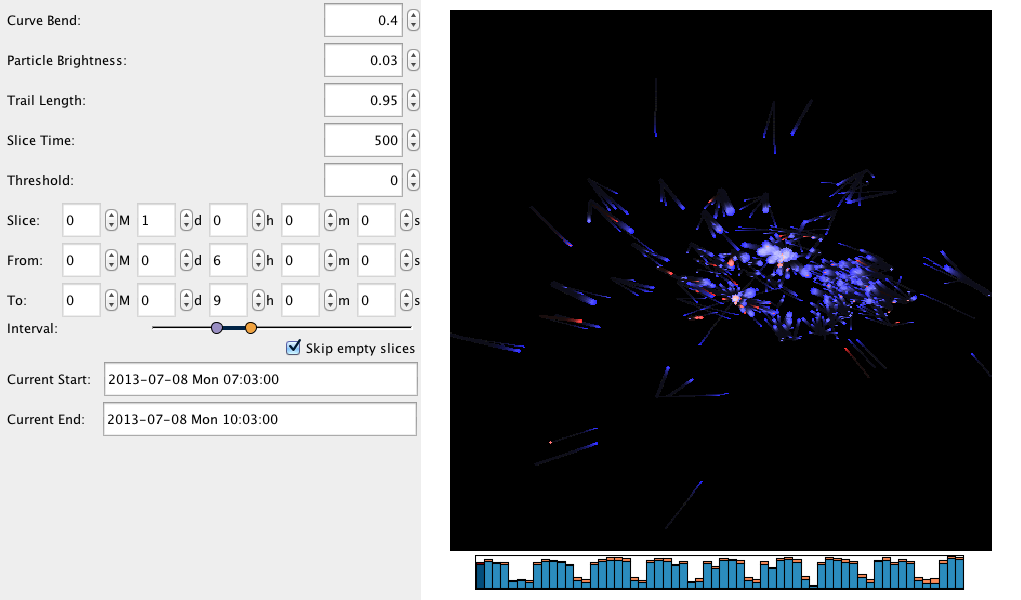
\includegraphics[width=0.9\linewidth]{images/tool.png}
\caption{The tool is split in three parts. On the right side is the
dot visualization. On the bottom right is the bar chart representation.
On the left is the control panel,
where the user can define the excursion of the trips, the brightness of
the dots, the length of the trails, the animation speed of the slices
and the threshold to remove dots that are too small.
With the spinners below this, the user can define the length of a slice and
the start and end of the relevant window.
The relevant window can also be edited by using the sliders below.
The user has also the option to skip slices that contain no trips, however
this only occurs when the duration of the slice is chosen very short.
The text fields at the bottom show the start and the end time of the
currently displayed relevant window.
}
\label{fig:tool}
\end{figure*}

\section{Data}
\label{sec:data}
The data used in this paper is provided by Capital~Bikeshare~\cite{wash}
the bike share company of Washington, DC. The data, reaching back
to October 2010, is freely available \cite{data}, though we used
only data from October 2012 until September 2013 to avoid the need
to skip the majority of the time to get to the latest data.
The remainder are 2470109 unique bicycle trips through Washington.

The trips are provided in multiple CSV files that vary in their format
per quarter.
Each trip consists of the name of the station where the bike was
picked up, the name of the station where the bike was put back, the time of
starting the trip, the duration, and whether the person was a
casual user or a subscribing member.
We processed the names of the stations,
usually consisting of the intersecting road names,
and converted them to geographic coordinates with a Geocoding
tool \cite{convert}.
We stored the trips in a MySQL database with the start time
as index to allow for fast ranged trip lookups by start time.

\section{The Tool}
\label{sec:impl}
In our tool we present trips as dots moving on a black background.
Every dot can be colored blue (indicating bike share subscription of the driver)
or red (indicating a casual user). The dots move on a curved path from
its origin to its destination to avoid over-plotting of opposing trips
similar to Wood~\etal\cite{Wood2011} and
Beecham~\etal\cite{Beecham2012}.
However, they cycle the animation of a given set of trips continuously,
whereas we split the time in slices and advance time constantly.
In our approach the complete data set is split into time slices of equal
length and within those slices we define a relevant window.
At the beginning of each time slice we create dots for trips of the
relevant window and start moving them. If a trip lasts longer than the
relevant window we let it continue to move during the next slice.

\begin{figure*}
\centering
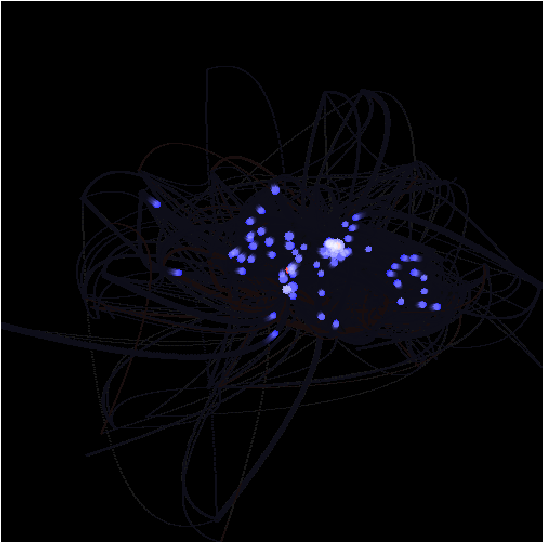
\includegraphics[width=3cm]{images/rush_7_tue.png}
\hspace*{0.5cm}
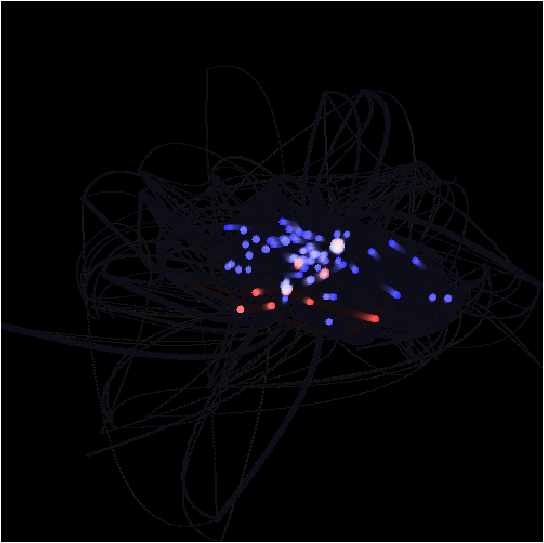
\includegraphics[width=3cm]{images/day_7_fri.png}
\hspace*{0.5cm}
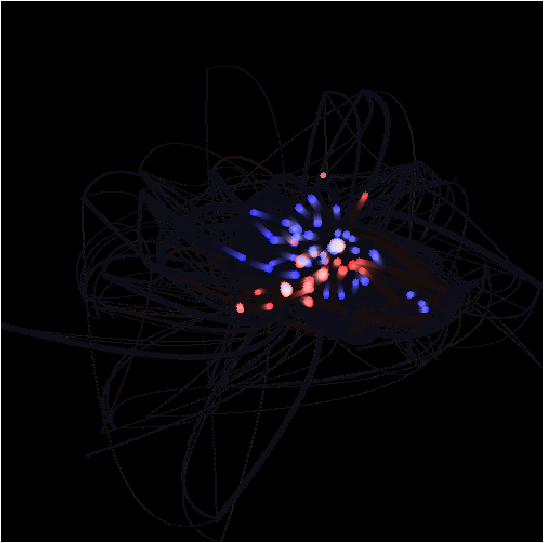
\includegraphics[width=3cm]{images/day_7_sun.png}
\hspace*{0.5cm}
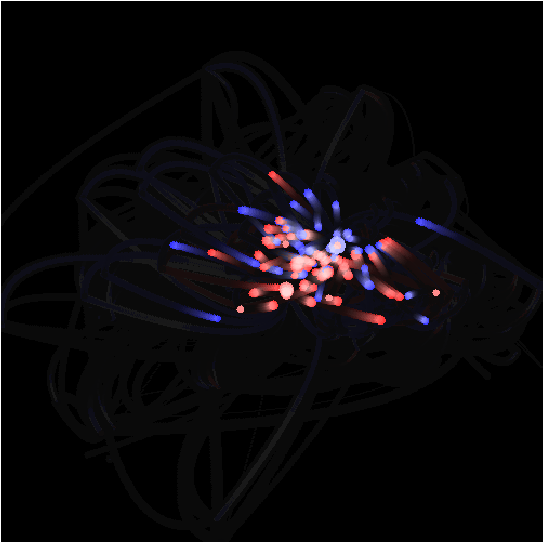
\includegraphics[width=3cm]{images/full_10_sun.png}
\hspace*{0.5cm}
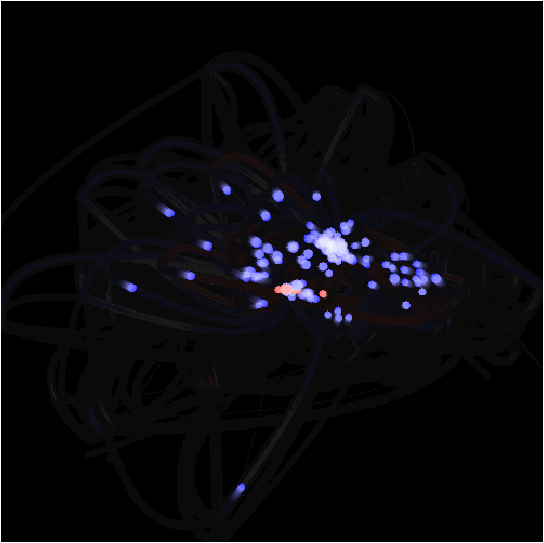
\includegraphics[width=3cm]{images/full_10_wed.png}
\caption{Different time slices. The leftmost image shows
bike usage during the morning rush hour, the second shows
bike usage during the day on a week day. The third image
shows bike usage during the day on a Sunday.
The last two images show the bike usage of two complete
days (relevant window is 24 hours), the first being a Sunday
and the second being a weekday. All images are during the summer months.}
\label{fig:smallm}
\end{figure*}

To make the vast number of simultaneous trips for longer slices
easier to read we aggregate similar trips based on origin, destination,
duration, and type. The aggregated trips are then represented as larger
dot.
Furthermore, we show a trail for each moving dot to make its
route easier to follow and gasp.
The user can vary those parameters when needed and can also
set a threshold of a minimal number of trips for a dot to be shown at all.

In addition to the animated trails the tool shows a summary of
future slices as bar chart.
The bar chart shows the total number of trips in the relevant window
of the given slices.
It starts with the currently displayed slice and shows the next 59 slices.
The blue part of the bar shows the number of subscriber trips during
the relevant window and the red part shows the number of casual users.

As further information about the current state the start and end times
of the current relevant window is always shown.
The complete tool can be seen in Figure~\ref{fig:tool}.
It is efficiently implemented using a MySQL database as storage and
OpenGL accelerated image blending to show the movement of the dots
and simulate their trails.
This allows for an interactive user experience with immediate feedback.

\begin{figure}[h]
\centering
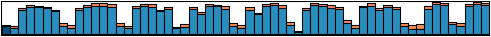
\includegraphics[width=\linewidth]{images/barchart.png}
\caption{The bar chart view showing the number of trips per relevant
window.
In this bar chart the slice length is one day, the relevant window is
during the morning rush hour.
Weekends can be easily identified by a decreasing number of trips
which sometimes start already on fridays.
The current (leftmost) slice is a Saturday.}
\label{fig:bar}
\end{figure}

\section{Results}
\label{sec:result}
By comparing trips during the morning rush-hour (time window from
6am to 9am) to trips during the day until the start of
the evening rush-hour (9am to 5pm) one can easily see
how different user groups use the bike sharing program.
See Figure~\ref{fig:smallm} for some snapshots.

The daily commuters during the rush hour have usually longer
journeys than users during the day. The commuters create
a temporary imbalance in the morning by bringing bicycles
to the center of the city where they work. However, the imbalance is
resolved in the evening during this rush hour. During the relatively
early time of the morning rush hour the number of casual users
is very low.

During the day the trips are much shorter and concentrate on the
center of the city. Casual users drive from the White House to
the Lincoln Memorial and vice versa implying this service is mainly
used by tourists visiting the city. The trips, however, are not
equally distributed in both directions which leads to slight (due to
the relatively small number) imbalance of bicycles in the touristy
area.

Comparing weekdays to weekends shows that during the weekend
the total number of trips far less than during the week (This can also
easily be seen by looking at the bar chart representation. See Figure~\ref{fig:bar}).
Also the ratio of casual users is much higher.
This is likely due to day tourists visiting over the weekend
and the working commuters staying at home on the weekend.
However, trips on a weekend are not as much focused on the center
as trips during the mid day on the week.
This may come from
people that normally do not use the bike share but use it on
weekends to get to the city.

\section{Future Work}
The tool can be expanded to show multiple views of different
relevant windows at once to make comparison easier.
Making the bar chart view clickable in order to directly jump to
a time slice would make navigation through the data set easier.
A cycle plot as used by Beecham~\etal\cite{Beecham2012}
can be used to show the distribution of trips within a slice
which would make it easier to choose the relevant window.

Also, using other data sets without fixed origins and destinations
can create new challenges of how to aggregate trips
effectively.


%% if specified like this the section will be committed in review mode
%\acknowledgments{}

\bibliographystyle{abbrv}
%%use following if all content of bibtex file should be shown
%\nocite{*}
\bibliography{trails}
\end{document}
